\chapter{Reinforcement Learning}\label{chap:reinforcement}

\chapterQuote{
    \textit{``One learns from books and examples only that certain things can be done. Actual learning requires that you do those things.''}\\
    }{--- Frank Herbert}

\chapterAbstract{R}{einforcement Learning (RL) encompasses all techniques that train intelligent agents in a simulated environment via rewards to perform actions that modify said environment in some way. In this chapter, we get an overview of how Reinforcement Learning operates and the different algorithms and techniques that have arisen. Section~\ref{sec:rl-intro} introduces Markov's Decision Process (MDP), which encompasses all RL problems. We also cover the elements found in every RL problem as well as how they interact with each other. Finally, we elucidate about the evolution of the different methods to perform Reinforcement Learning training. This chapter is sectioned as follows Section~\ref{sec:rl-algorithms_and_techniques} showcases the evolution of RL algorithms throughout the years and reward implementations that became standardized. Section~\ref{sec:rl-applications} shows some applications for Reinforcement Learning. Finally, Section~\ref{sec:rl-summary} summarizes all the information given.}


\section{Introduction}\label{sec:rl-intro}
Machine learning is a subfield of artificial intelligence that focuses on the development of algorithms and models that can learn from data. There are three main types of machine learning: supervised learning, unsupervised learning, and reinforcement learning. In supervised learning, the algorithm is trained on a labeled dataset, where the input data is associated with a corresponding output label. The goal of supervised learning is to learn a mapping from input to output that can generalize to new, unseen data. In unsupervised learning, the algorithm is trained on an unlabeled dataset, where the goal is to discover patterns and structure in the data. Unsupervised learning can be used for tasks such as clustering\cite{}, dimensionality reduction\cite{}, and anomaly detection\cite{}.

Reinforcement learning is a type of machine learning that is used to solve problems where the agent interacts with an environment and receives feedback in the form of rewards. The goal of reinforcement learning is to learn a policy that maximizes the cumulative reward over time. Reinforcement learning is particularly useful for problems where the optimal action depends on the current state of the environment and the actions taken in the past. Reinforcement learning has been successfully applied to a wide range of problems, including robotics\cite{}, game playing\cite{}, recommendation systems\cite{}, and other areas.

Reinforcement learning is different from supervised and unsupervised learning in several ways. In supervised learning, the algorithm is provided with labeled data, whereas in reinforcement learning, the algorithm learns from feedback in the form of rewards. In unsupervised learning, the algorithm is trained on an unlabeled dataset, whereas in reinforcement learning, the algorithm interacts with an environment. Reinforcement learning also requires a different evaluation metric than supervised and unsupervised learning, since the goal is to maximize the cumulative reward over time rather than to minimize a loss function.

Reinforcement Learning techniques need to adapt to real-world environments, which is a challenging task given that reality is often diverse, non-stationary and open-ended. RL is generally described as having low generalization, i.e., it is hard to create general-purpose agents. This, in turn, generates another problem: environmental overfitting. Trained agents specialize in the environment in which they were trained and are very susceptible to small changes, needing to be re-trained very often when new knowledge is added\cite{}.

\subsection*{Markov Decision Process}
Markov decision processes (MDPs) are stochastic decision-making processes that use a mathematical framework as model. MDPs provide a formal framework for modeling situations where outcomes are partly random and partly under the control of the decision-maker. 

MDPs were introduced in the 1950s by Russian mathematician Andrey Markov who played a pivotal role in shaping stochastic processes. In their infancy, MDPs were used to solve business-related problems such as inventory management and control, queuing optimization, and routing matters. Today, MDPs find applications in studying optimization problems via dynamic programming, robotics, automatic control, economics or manufacturing.

In an MDP, the decision maker, or agent, interacts with an environment that is characterized by a set of states, actions, and rewards. The agent's goal is to learn a policy that maximizes the cumulative reward over time.

\begin{figure}[!htp]
    \centering
    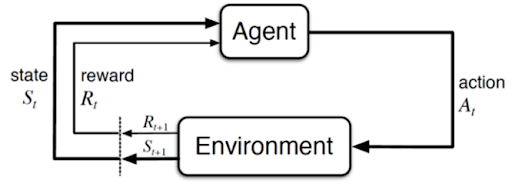
\includegraphics[width=.6\textwidth]{fig/rl/MDP-model.png}
    \caption{A Markov decision process loop.}
    \label{fig:MDP}
\end{figure}

The future state of the environment depends only on the current state and action, and not on the history of previous states and actions. This is known as the Markov property. This way the agent can use the current state of the environment to estimate the expected future rewards of different actions, and then choose the action that is most likely to lead to the highest cumulative reward over time.

Based on the notation from figure \ref{fig:MDP}, the Markov property can be evaluated as shown in Equation \ref{eq:markov_property}.

\begin{equation}
    \label{eq:markov_property}
    P[St+1|St] = P[St+1|S1,S2,S3,.....,Sn]
\end{equation}

Where the probability of the next state (P[St+1]) given the present state (St) is calculated based on all the possible next states (S1, S2, S3,\dots, Sn).
The relation between the action to be chosen and the chosen outcome reward is referred to as the policy ($\pi$), $\pi: S -> A$.

To determine the best policy, it is essential to obtain optimal values produced for the agent's rewards at every state. The discount factor ($\gamma$) [0-1] determines which rewards are prioritized, minimal values focus on immediate rewards while maximum values focus on long-term rewards. The discounted infinite-horizon method expressed by the value function in Equation \ref{eq:value_function} determines the reward for each state by discounting future rewards.

\begin{equation}
    \label{eq:value_function}
    V(s) = E \sum_{t=1}^{\inf}\gamma^t r_t|s_t
\end{equation}

This value function can be separated into two components as shown in equations \ref{eq:vf1} and \ref{eq:vf2} which showcases the joint equation with both states and the split equation for the current and next states respectively.

\begin{equation}
    \label{eq:vf1}
    V(s) = E [r + \gamma V(s_{t+1})|s]
\end{equation}

\begin{center}
    $\Downarrow$
\end{center}

\begin{equation}
    \label{eq:vf2}
    V(s) = \mathcal{R}_s + \gamma \sum_{s_{t+1} \in S}^{\inf}\gamma^t r_t|s_t
\end{equation}

% \begin{figure}[!h]
%     \centering
%     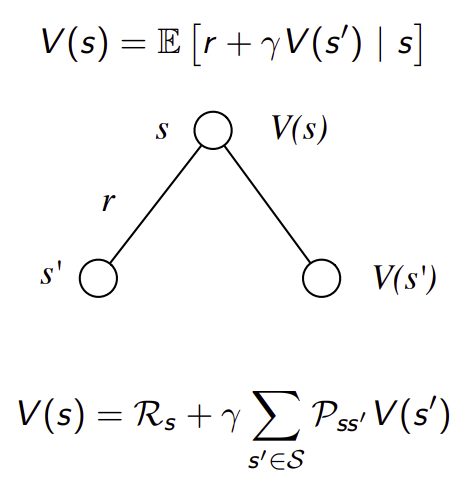
\includegraphics[width=.4\textwidth]{fig/rl/Bellmans decomposition.png}
%     \caption{Value function equation decompostion}
%     \label{fig:bellman}
% \end{figure}

or in other words, the reward for the current state and the value of the discounted reward for the next state. Furthering this line we arrive at  Bellman's Equation (\ref{eq:bellmans}).

\begin{equation}
    \label{eq:bellmans}
    V(s) = max_a[ \mathcal{R}(s,a) + \gamma \sum_{s_{t+1} \in  S}\mathcal{P}_{ss_{t+1}} V(s_{t+1})]
\end{equation}

Where $s_{t+1}$ represents the next possible state, $s$ the current state, $\mathcal{P}_{ss_{t+1}}$ the probability of transitioning to $s_{t+1}$  based on the reward ($\mathcal{R}(s,a)$) for choosing action $a$.

The agent's actions and rewards vary based on the policy chosen for training, manifesting that the value function is different for each one. choosing the right policy is a type of operation that can be solved by iterative methods such as Monte Carlo evaluations, dynamic programming, or temporal-difference learning. The policy that selects the maximum optimal value while considering the present state is referred to as the optimal policy as seen in Equation \ref{eq:optimal_policy}

\begin{equation}
    \label{eq:optimal_policy}
    \pi(s) = argmax_a[\mathcal{R}(s,a) + \gamma \sum_{s_{t+1} \in S}\mathcal{P}_{ss_{t+1}}^a V(s_{t+1})]
\end{equation}

The policy is, in essence, a particular application of Bellman's equation for each step, a new policy is evaluated based on the current state information.

\subsection*{Reinforcement Elements}

Reinforcement Learning can be defined as a Markov process that solves policy optimization functions by using Neural Networks for this reason RL problems are considered substrata of Markov's processes, and as such share a multitude of elements with them, for instance, the States, Actions, Environment, and Agent interactions while also being respectful of Markov's Property. As Sutton and Barto put it, they are an "optimal control of incompletely-known Markov decision processes\cite{sutton2018reinforcement}".

Some core elements of RL problems are as follows:

\begin{itemize}
    \item A learning agent must be able to sense the state of its environment to some extent and must be able to take actions that affect the state.
    \item The agent also must have a goal or goals relating to the state of the environment.
    \item In supervised learning the agent learns from a labeled training set in order to extrapolate future answers not present on it. In RL agents must be able to learn from their own experience as when dealing with interactive problems it is often impractical to obtain examples of desired behavior that are both correct and representative of all the situations in which the agent has to act.
    \item Reinforcement learning differs from unsupervised learning, one istries to maximize a reward signal instead while the other focuses on finding a hidden structure.
\end{itemize}

A key difference between RL and other types of learning is the exploration/exploitation dilemma: RL favors actions that provide high rewards (exploitation), but in order to reach the intended solution it may have to select low-reward actions in the early stages of training or actions that have not been selected before (exploration). The dilemma is that neither exploration nor exploitation can be pursued exclusively without failing at the task. The agent must try a variety of actions and progressively favor those that appear to be best.

The elements of reinforcement Learning as we have previously commented are similar to MDPs. Sutton and Barto\cite{}, apart from the environment and agent enumerate the following elements:

\begin{itemize}
    \item The \textbf{policy} is the "brain" of the decision-maker in Markov's processes, an action mapping acquired from the perception of the agent from the current state of the environment that determines which action should be taken.
    
    \item The \textbf{reward signal} is the goal the Agent is trying to reach. Each action chosen by the Agent during training receives a numerical reward that must be maximized. It determines what constitutes a good or bad event while the agent learns and thus shapes its behavior. In general, reward signals may be stochastic functions of the state of the environment and the taken actions.
    
    \item The \textbf{value function} helps the agent determine what a good course of action to follow is in the long run. Value of a state is the total amount of reward an agent can expect to accumulate over the future, starting from that state. values indicate the long-term desirability of states after taking into account the states that are likely to follow, and the rewards available in those states
     
    \item Some RL systems rely on a \textbf{environment model}, which is a predictor for how the environment will behave, given a state and action the model can approximately predict the next state and reward for that action. Some RL systems plan ahead and gather information about future states without actually experiencing them. these model-based methods contrast with the purely experience-based methods that originated RL.
\end{itemize}

\subsection*{History}
The roots of reinforcement learning can be traced back to early 20th-century psychologists like Thorndike\cite{} and Skinner\cite{}, who laid the groundwork for the concept of reinforcement by studying animal behavior.

In the 1950s and 1960s, control theory, which deals with the behavior of dynamic systems, influenced the development of reinforcement learning. Bellman's work on dynamic programming and optimal control provided a mathematical framework, introducing the Bellman equation as we previously discussed in equation \ref{eq:bellmans}.

Computer scientists in the mid-20th century explored ways to make machines learn from experience. Samuel's 1959 checkers-playing program, which employed temporal difference learning\cite{}, demonstrated that machines could attain expertise in games without explicit programming. The 1980s saw the development of algorithms capable of learning from delayed rewards, including the widely-used Q-learning introduced by Watkins in 1989 \cite{}.

The 1990s saw the convergence of reinforcement learning with neural networks, giving rise to deep reinforcement learning. Tesauro's TD-Gammon in 1995 showcased the potential of this combination by achieving expert-level play in backgammon\cite{}. In the 21st century, breakthroughs in deep reinforcement learning have been remarkable, exemplified by DeepMind's 2013 Deep Q-Network (DQN) algorithm\cite{}.

From its origins in psychology to its current status as a powerful AI tool, the evolution of reinforcement learning has been marked by significant milestones and breakthroughs that are still ongoing. The following section will provide further details about the aforementioned proposals and study their evolution.

\section{Algorithms and Techniques}\label{sec:rl-algorithms_and_techniques}
This section will give an overview of each key evolution in RL development, as previously mentioned control theory is the origin of RL development, by evaluating and trying to solve dynamic systems, A. L. Samuel introduced Temporal Difference Learning \cite{samuel1959checkers} in a checkers game context, it is a type of reinforcement learning algorithm that updates the estimated value of a state based on the difference between the value of the next state and the current state, this difference is referred to as the TD-error.

Rather than aiming to compute the overall future reward on each step, the algorithm compares the new prediction with the previously stored one. If there is a disparity between the two predictions, the TD Learning algorithm quantifies this difference and employs it to update the previous prediction to the new one.

TD algorithms are based on Bellman equations, it computes optimal policies by recursively computing the value of each state. This way the algorithm is able to learn from incomplete sequences of experience, where the final outcome is not known at the time of the update, this was a significant improvement in reward prediction and paved the way for more modern RL approaches. 

Q-learning, developed by Watkins et. al. \cite{} in 1989, follows a similar methodology to that of TD learning, which updates the value of a state based on the difference between the value of the next state and the current state, Q-learning updates the value of a state based on the maximum value of the next state. The objective of Q-learning is to calculate an approximation \textit{Q} of the optimal action-value function \textit{q*} which is independent of the policy and store these updates in a table of action-value pairs called the Q-table. This makes Q-learning an off-policy algorithm, as it learns the optimal action-value function \textit{Q} regardless of the policy being followed. This action-value function is shown in equation \ref{eq:q-learning_value_function}.

\begin{equation}
    \label{eq:q-learning_value_function}
    Q(S_t, A_t) \leftarrow Q(S_t, A_t) + \alpha [R_{t+1} + \gamma max_a Q(S_{t+1}, a) - Q(S_t, A_t)]
\end{equation}

Where $\alpha \in (0,1]$ is the step size, $S_t$ is the state in timestep t, $A_t$ the action in timestep t, $\gamma$ is the discount factor of rewards for update, and $R_{t+1}$ the expected reward for the action chosen.

Even though Q-learning is an off-policy method, the policy still has an effect, it determines which states and actions to pick and evaluate for every episode. Q-learning works by iteratively updating the estimated value of a state-action pair based on the difference between the estimated value and the actual return obtained from taking that action in that state. The algorithm starts with an initial estimate of the action-value function and iteratively updates the estimates based on the observed returns. The algorithm continues to update the estimates until the action-value function converges to the optimal values as seen in figure \ref{fig:Q-learning}.

\begin{figure}[!h]
    \centering
    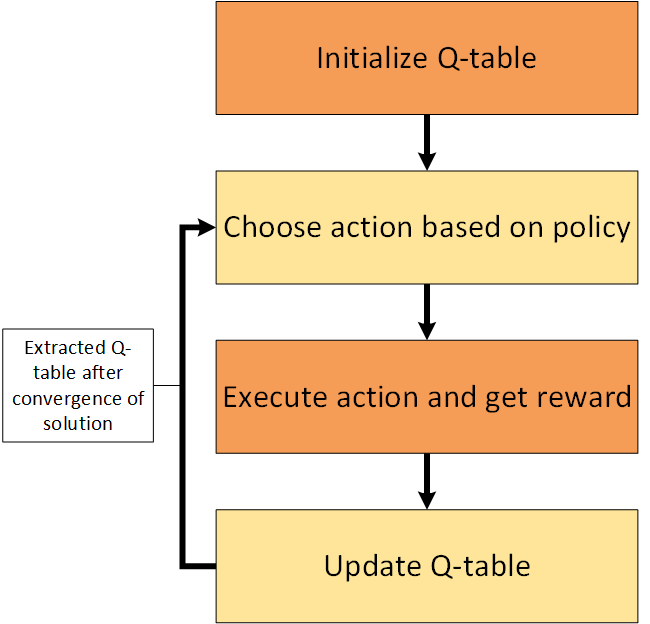
\includegraphics[width=.5\textwidth]{fig/rl/Q-learning.png}
    \caption{Q-learning operations diagram}
    \label{fig:Q-learning}
\end{figure}

One of the main advantages of Q-learning is that it can be used to learn optimal policies in environments with large or continuous state and action spaces. This is because Q-learning does not require a model of the environment, but rather learns from experience by iteratively updating the action-value function.

In the 1940s, John von Neumann and Stanislaw Ulam introduced the Monte Carlo method named after Monaco's famous casino, due to its reliance on randomness akin to a game of roulette.

Monte Carlo's methods estimate the value of a state or action based on the average return obtained by sampling complete episodes, unlike TD learning, which updates every step by comparison to previous results.

Monte Carlo methods use the actual return obtained from the episode to update the value of the states in that episode based on the actions taken, they are particularly useful in situations where the dynamics of the environment are unknown or stochastic, as they do not require a model of the environment, instead, they rely on experience to estimate the value of each action-state pair.

\begin{figure}[!h]
    \centering
    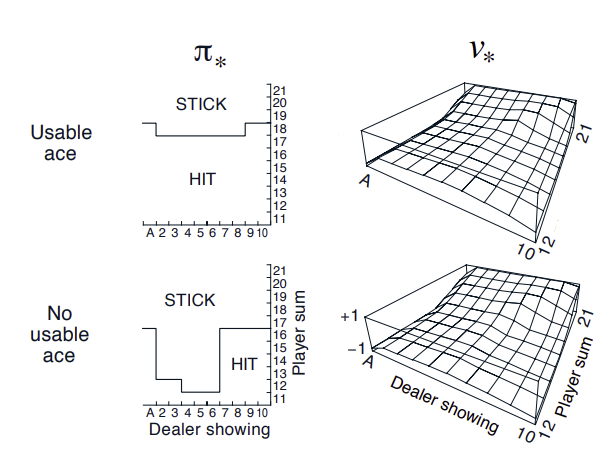
\includegraphics[width=.7\textwidth]{fig/rl/Monte Carlo Blackjack convergence.png}
    \caption{The game of blackjacks policy and value function as calculated by following a Monte Carlo control approach}
    \label{fig:monte-carlo}
\end{figure}

Monte Carlo methods work by simulating complete episodes of interaction between the agent and the environment, starting from a given state and following a given policy (Off-policy Monte Carlo methods aside) this particular method of applying Monte Carlo to control theory is generally referred to as Monte Carlo control, Figure \ref{fig:monte-carlo} shows the calculation of the policy and value function for a simplified game of blackjack.

The return obtained from each episode is then used to update the value of the states and actions that were visited for that episode. This process is repeated many times, with the value estimates converging to the true values as the number of episodes increases. Monte Carlo methods are unbiased and consistent, meaning that they converge to the true values of the states or actions with probability 1 as the number of episodes goes to infinity.

One of the main advantages of Monte Carlo methods is that they can be used to estimate the value of any state or action, regardless of its position in the state space or action space. This makes them particularly useful in large or continuous state and action spaces.

In contrast to the previous methods, the more modern Policy Gradient Methods differ from the previous approaches in that they do not focus on learning the values of actions to then select the highest one, instead, Policy Gradient Methods learn a parameterized policy that can select actions without consulting a value function (equation \ref{eq:policy_gradient}), however, a value function may be applied to learn the policy ($\pi$) but is not required for action selection.

\begin{equation}
    \label{eq:policy_gradient}
    \pi(a|s,\theta) = Pr\{A_t=a | S_t=s, \theta_t=\theta\}
\end{equation}

Where $\theta$ represents the policy parameters, a is the probability of that action being taken, in timestep t for the current state s.

This parametrized policy function takes the current state of the environment as input and outputs a probability distribution over possible actions. During training, the agent interacts with the environment, taking action according to its current policy. The rewards obtained from these actions are used to adjust the parameters of the policy function through a process called gradient ascent, this process is as follows:

\begin{itemize}
    \item If an action leads to a higher reward, the probability of taking that action in similar future situations is increased.
    \item If an action results in a lower reward, the probability of taking that action is decreased.
    \item This adjustment is guided by the gradient of the expected cumulative reward with respect to the policy parameters.
    \item Iteratively updating the policy based on this gradient, the agent learns to make better decisions over time, improving its performance in the given environment.
\end{itemize}

Policy gradient methods learn the policy parameter $\theta$ based on the gradient of some performance measure $J(\theta)$ linked to the policy parameter and seek to maximize this performance measure as depicted in equation \ref{eq:gradient_ascent}.

\begin{equation}
    \label{eq:gradient_ascent}
    \theta_{t+1} = \theta_t + \alpha \nabla J (\theta_t)
\end{equation}

Where $\nabla J (\theta_t)$ is an approximation of the gradient of performance $J(\theta)$ for the timestep t and $\alpha$ is the learning rate a parameter to control the speed of the agent learning. All methods that follow this methodology of approximating a gradient for performance linked to a parametrized policy are what encompasses policy gradient methods, they offer flexibility and can handle high-dimensional action spaces, making them well-suited for complex tasks. However, training can be computationally intensive, requiring multiple interactions with the environment to fine-tune the policy.

The action selection in policy gradients is a stochastic event, where the probability of an action is computed as the estimated reward for the state that action leads to, making the process a stochastic gradient ascent.

The REINFORCE \cite{sutton1999policy} is the first policy-gradient-based algorithm that follows this stochastic gradient ascent method. The main idea behind it is to maximize the expected cumulative reward by adjusting the parameters of the policy $\theta$ in the direction that increases the likelihood of actions leading to higher rewards so that it learns to take them. In other words, it maximizes the policy gradient function $\nabla J (\theta_t)$ by finding the optimal $\theta$ for the maximization of $J(\theta)$, formally defined by equation \ref{eq:gradient_ascent_rein}.

\begin{equation}
    \label{eq:gradient_ascent_rein}
    \nabla_\theta J(\theta) = \mathcal{E}_\pi[\sum_{t=0}^{inf}\nabla_\theta log \pi(a_t|s_t;\theta)G_t]
\end{equation}

$G_t$ is the return at timestep t, identified by equation \ref{eq:expected_return_reinforce}

\begin{equation}
    \label{eq:expected_return_reinforce}
    G_t = \sum_{k=0}^{\inf} \gamma^k R_{t+k+1}
\end{equation}

$\nabla_\theta log \pi(a_t|s_t;\theta$ is the score function representing the gradient of the log probability of taking action $a_t$ in state $s_t$ with respect to the policy parameters $\theta$, REINFORCE then updates the policy parameter and performs stochastic gradient ascent as seen in previous equation \ref{eq:gradient_ascent}. The key intuition is that the policy parameters are adjusted in proportion to the gradient of the expected return, encouraging actions that lead to higher rewards to become more likely.

REINFORCE shares similarities with Monte Carlo processes, particularly in how it estimates expected values. In both REINFORCE and Monte Carlo methods, an agent interacts with the environment over a sequence of steps and receives a cumulative reward at the end of each episode. Instead of directly calculating the expected cumulative reward, both approaches estimate it by sampling multiple trajectories (sequences of states, actions, and rewards) and averaging the observed returns.

REINFORCE, in comparison to traditional Monte Carlo methods, offers the key improvement of leveraging policy gradients, enabling the algorithm to handle continuous action spaces and apply parametrized policies, often implemented with neural networks. The probabilistic nature of REINFORCE facilitates effective exploration strategies, reducing variance in estimated returns and promoting stable convergence during training.

Actor-critic methods represent a class of reinforcement learning algorithms that combine elements of both policy-based (actor) and value-based (critic) approaches. The fundamental idea is to have two distinct components within the learning agent: an \textbf{actor} that learns a policy to select actions, and a \textbf{critic} that evaluates the value of state-action pairs. This dual structure allows for more efficient learning and improved stability compared to pure policy or value-based methods.

The actor update function uses the policy gradient of the expected cumulative reward with respect to the policy parameters, which we have previously explored in REINFORCE (eq. \ref{eq:gradient_ascent_rein}) without the expected return $G_t$, and instead relying on an advantages function $Q(s,a)$ that represents the difference between the estimated value of a state-action pair and the value function only in the evaluated state as shown in equation \ref{eq:gradient_actor_critic}. 

\begin{equation}
    \label{eq:gradient_actor_critic}
    \nabla_\theta J(\theta) \eqsim \mathcal{E}_\pi[\nabla_\theta log \pi(a_t|s_t;\theta)Q(s,a)]
\end{equation}

The critic parameters $\mathcal(w)$, and $\beta$, the critic's learning rate, are updated using TD learning methods. the critic tries to approximate the TD error $\delta$ between the estimated value $V(s_t;\mathcal(w))$ and the current cumulative reward $R_{t+1}$ plus the discounted value of the next state $\gamma V(s_{t+1};\mathcal(w))$, formally described by equation \ref{eq:td-error_critic}.

\begin{equation}
    \label{eq:td-error_critic}
    \delta = R_{t+1} + \gamma V(s_{t+1};\mathcal(w)) - V(s_t;\mathcal(w))
\end{equation}

The TD error measures the difference between the agent's prediction of the immediate reward and its estimate of the future rewards, providing a signal for updating the critic's parameters, which are updated by using the gradient of the TD-error with respect to the critic's parameters $\mathcal(w)$ according to the learning rate $\beta$, formally described by equation \ref{eq:parameter_update_critic}.

\begin{equation}
    \label{eq:parameter_update_critic}
    \mathcal(w)_{t+1} = \mathcal(w)_t + \beta \nabla_\mathcal(w) \delta V(s_t;\mathcal(w))
\end{equation}

This equation reflects the iterative adjustment of the critic's parameters to minimize the TD error, aligning the predicted values with the observed rewards. The learning rate ($\beta$) determines the step size in the parameter space.

Actor-critic methods strike a balance between exploration (through the actor's policy) and exploitation (through the critic's value estimates), reducing the variance caused by policy gradient Monte Carlo methods.

\section{Applications}\label{sec:rl-applications}
This section provides a concise exploration of diverse applications harnessing the power of reinforcement learning (RL). From gaming to Autonomous driving or Industrial control, RL exhibits its versatility by optimizing decision-making processes across an array of domains.

\subsection*{Games}
Whether in traditional board games or cutting-edge video games, reinforcement learning has demonstrated remarkable prowess in mastering strategic decision-making and optimizing gameplay. These approaches showcase the evolution of AI's gaming capabilities and their broader implications.

AlphaGo\cite{silver2016mastering} represents a groundbreaking application of reinforcement learning in the realm of board games, specifically Go. Developed by DeepMind, AlphaGo employs a combination of deep neural networks and Monte Carlo Tree Search to navigate the immense complexity of the game. Its neural network-based policy and value functions enable strategic decision-making, while the Monte Carlo Tree Search facilitates lookahead exploration. Notably, AlphaGo's triumph over human champion Fan Hui marks a turning point in machine learning history, showcasing the capability of reinforcement learning to master complex strategic domains with profound implications for artificial intelligence and game theory research.

AlphaZero\cite{silver2017mastering} extends the paradigm established by AlphaGo, utilizing a reinforcement learning approach for mastery in a broader spectrum of board games, including chess and shogi. AlphaZero relies solely on self-play reinforcement learning without access to human game data or domain-specific knowledge. Its unparalleled success in surpassing world-champion level performance across multiple games displays the ability of RL to achieve superhuman proficiency and generalization within strategic gaming domains.

However, AlphaStar\cite{vinyals2019grandmaster} marks a notable advancement in the application of reinforcement learning, applying similar techniques for real-time strategy games. Leveraging a combination of deep neural networks and a unique multi-agent training setup, AlphaStar achieves superhuman proficiency in StarCraft II, surpassing top human players. Its capacity to handle the complexity of real-time decision-making within the game environment underscores the robustness and scalability of reinforcement learning methodologies in addressing challenges beyond turn-based or board game scenarios.

\subsection*{Industrial Control}
But Reinforcement learning can be applied to much more than games, it proves its versatility in addressing real-world challenges, For example in the world of controlling operations in industrial processes.

For instance, in data center cooling, by enhancing safety and efficiency within critical infrastructure settings, Traditional control systems often struggle to adapt dynamically to complex and changing environments, leading to inefficiencies and potential safety risks. by leveraging RL techniques significant energy savings and reducing CO2 emissions to help combat climate change become a reality.

The approach works by polling the server sensors continuously and feeding the information given by these sensors to deep neural networks, which predict how different actions will affect future energy consumption. The system identifies how to minimize energy consumption and maintain satisfactory safety constraints. Those actions are sent back to the data center, where the actions are verified by the local control system and then implemented.

Other techniques in industrial control came with new interests in Nuclear fusion, new tokamak designs in toroidal shapes have been produced and Reinforcement Learning provided a way to optimize the magnetic polarity to maintain the temperature inside these machines \cite{degrave2022magnetic}.

RL has produced and controlled a diverse set of plasma configurations for the Tokamak and achieves accurate tracking of the location, current and shape of these configurations. This represents a notable advance for tokamak feedback control, showing the potential of reinforcement learning to accelerate research in the fusion domain, and is one of the most challenging real-world systems to which reinforcement learning has been applied.

\subsection*{Autonomous Driving}
Autonomous driving presents a transformative shift in transportation that holds immense potential to enhance our lives. The promise of significantly improved safety on the roads, with autonomous vehicles minimizing human errors and reducing traffic accidents. 

Beyond safety, autonomous driving has the capacity to enhance accessibility for individuals facing transportation challenges, fostering independence and inclusivity. The technology's potential to optimize traffic flow promises more efficient and less congested road networks, translating to reduced travel times and environmental impact. 

Moreover, the prospect of increased productivity and improved quality of life emerges as individuals can utilize travel time for work or relaxation. The evolution of urban planning and space utilization, prompted by autonomous driving, may lead to more sustainable and pedestrian-friendly cities. While challenges persist, the multifaceted benefits of autonomous driving suggest a future where transportation becomes safer, more efficient, and enriching for individuals and communities alike.

Multiple methods exist that leverage reinforcement Learning for controlling vehicles automatically, they approach multiple tasks such as Intent prediction for traffic actors such as pedestrians or other vehicles \cite{}, path planning and trajectory optimization\cite{}, development of high-level driving policies for complex navigation tasks\cite{},  scenario-based policy learning for highways\cite{}, merges and splits\cite{}, intersections\cite{}, motion planning and dynamic path planning\cite{}, controller optimization\cite{}, learning of policies that ensures safety and perform risk estimation\cite{}.

\section{Summary}\label{sec:rl-summary}
The contents of this chapter have provided an overview of the methods improvements and applications of reinforcement learning in multiple contexts, We first learned about Markov processes and how RL fell under this umbrella, the elements that compose a reinforcement learning problem and the history of the methods that improved general RL. Then we learned about the algorithms at the core of RL and how each one improved upon the shortcomings of the previous ones. Finally, we observed some applications of RL to real-world problems.

